% !TEX encoding = UTF-8
% !TEX TS-program = pdflatex
% !TEX root = ../tesi.tex

%**************************************************************
\chapter{Progettazione e codifica}
\label{cap:progettazione-codifica}
%**************************************************************

\intro{Il seguente capitolo descrive gli strumenti e la progettazione con cui sono 
state implementate le integrazione con la \textit{web-app} \productName.}\\

%**************************************************************
\section{Tecnologie}
\label{sec:tecnologie-strumenti}

Di seguito viene data una panoramica delle tecnologie e strumenti utilizzati.

\subsection*{Java}
Java è un linguaggio di programmazione e una piattaforma di elaborazione 
rilasciato per la prima volta da Sun Microsystems nel 1995. Si è evoluto da umili
 origini per sostenere gran parte del mondo digitale di oggi, fornendo una
 piattaforma affidabile su cui sono costruiti molti servizi e applicazioni. 
 Anche i nuovi prodotti, innovativi nei servizi digitali progettati per il futuro,  
 continuano a fare affidamento su Java.
%TODO: aggiungere bibliografia, link: https://java.com/en/download/help/whatis_java.html
\subsection*{Spring}
Spring è un \textit{framework} open source per lo sviluppo di applicazioni su piattaforma Java.
A questo \textit{framework} sono associati tanti altri progetti, che hanno nomi composti come 
Spring Boot, Spring Data, Spring Batch, etc. Questi progetti sono stati ideati per
fornire funzionalità aggiuntive al \textit{framework}.
%TODO: aggiungere bibliografia, link: https://it.wikipedia.org/wiki/Spring_Framework

\subsection*{Typescript}
%**************************************************************
TypeScript è un linguaggio di programmazione sviluppato e gestito da Microsoft. 
È un \gls{superset} di JavaScript, che permette di aggiungere la tipizzazione 
statica opzionale al linguaggio. TypeScript è progettato per lo sviluppo di applicazioni 
di grandi dimensioni e per la \gls{transcompilazione} in JavaScript. Poiché TypeScript è un \gls{superset} di JavaScript, anche i programmi JavaScript esistenti sono validi programmi TypeScript.
%TODO: aggiungere bibliografia, link: https://en.wikipedia.org/wiki/TypeScript

\subsection*{Angular}
%**************************************************************
Angular è un \textit{framework} JavaScript per applicazioni \textit{web} dinamiche, utilizzato in particolare per la creazione di \gls{spa} e \textit{web-app}. Consente di utilizzare HTML come linguaggio template e di estenderne la sintassi per esprimere le componenti di un'applicazione in modo chiaro e succinto.
%TODO: aggiungere bibliografia, link: https://psicografici.com/angular-js/#:~:text=Angular%20%C3%A8%20un%20framework%20JavaScript,in%20modo%20chiaro%20e%20succinto.

\subsection*{Angular Material}
%**************************************************************
Angular Material è una libreria sviluppata da Google nel 2014 progettata per aiutare a sviluppare pagine \textit{web} in modo strutturato. \\
I suoi componenti aiutano a creare pagine \textit{web} e applicazioni \textit{web} attraenti, coerenti e funzionali.
%TODO: aggiungere bibliografia, link: https://psicografici.com/angular-js/#:~:text=Angular%20%C3%A8%20un%20framework%20JavaScript,in%20modo%20chiaro%20e%20succinto.

\subsection*{Node.js}
Node.js è una piattaforma di sviluppo open source per l'esecuzione di codice JavaScript lato \textit{server}. Node è utile per sviluppare applicazioni che richiedono una connessione permanente dal \textit{browser} al \textit{server} ed è spesso utilizzato per applicazioni in tempo reale come chat, feed di notizie e di notifiche.\\
Node.js è utilizzato da Angular per gestire le dipendenze, permettendo la dichiarazione di due insiemi di dipendenze: per gli sviluppatori e per far funzionare l'applicativo. In questo modo è possibile differenziare quali librerie si possono tralasciare in fase di \textit{deploy} dell'applicazione perché, ad esempio, necessarie solo per effettuare i test.
%TODO: aggiungere bibliografia, link: https://whatis.techtarget.com/definition/Nodejs#:~:text=James%20Denman-,Node.,feeds%20and%20web%20push%20notifications.

%**************************************************************
\section{Progettazione}
\label{sec:progettazione}

\subsection{Back-end}
\subsubsection{Architettura Spring Boot}
Spring Boot è un modulo di Spring \textit{framework}. Viene utilizzato per creare applicazioni \textit{stand-alone} di livello produttivo con il minimo sforzo.\\
Spring Boot segue un'architettura a strati, in cui ogni livello comunica con gli strati vicini.\\
Ci sono quattro strati in Spring Boot sono i seguenti:
\begin{itemize}
    \item \textbf{\textit{Presentation layer}:} gestisce le richieste HTTP, trasforma il il parametro da formato JSON in classe e autentica la richiesta, per poi trasferirla al \textit{business layer};
    \item \textbf{\textit{Business Layer}:} gestisce tutta la \textit{business logic}. Consiste in classi di servizio e utilizza servizi forniti dagli strati di accesso ai dati;
    \item \textbf{\textit{Persistence Layer}:} contiene tutta la \textit{storage logic}, e trasformando gli oggetti provenienti dalla \textit{business logic} in righe del \textit{database};
    \item \textbf{\textit{Database Layer}:} in questo strato sono effettuate le operazioni \gls{CRUD}.
\end{itemize}
\begin{figure}[H] 
    \centering 
    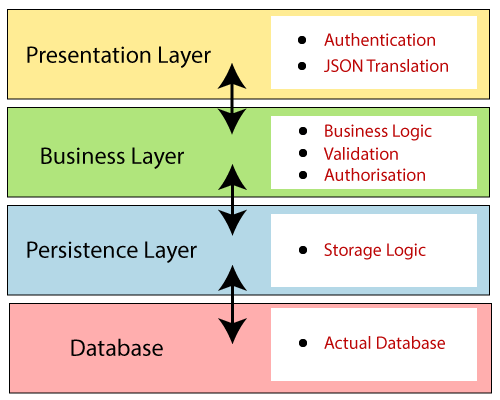
\includegraphics[scale=0.3]{spring-boot-architecture-layer.png} 
    \caption{Architettura a strati di Spring Boot}
\end{figure}

\subsubsection{Spring Boot Flow Architecture}
% https://codingjam.it/microservizi-in-java-con-spring-boot-e-spring-cloud/
\begin{figure}[H] 
    \centering 
    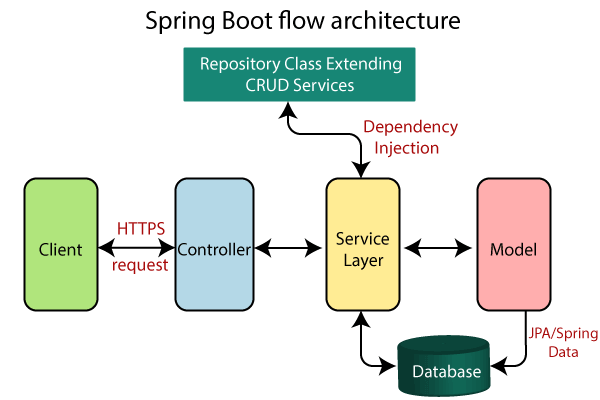
\includegraphics[width=1\columnwidth]{spring-boot-architecture.png} 
    \caption{Spring Boot \textit{workflow}}
\end{figure}
Il \textit{workflow} con cui vengono effettuate richieste HTTP utilizzando Spring Boot è il seguente:
\begin{itemize}
    \item il client esegue una richiesta HTTP (GET, POST, PUT O DELETE) ad un   \gls{endpoint} esposto;
    \item la richiesta va al \textit{controller}, che mappa la richiesta e la gestisce. Dopodiché chiama la \textit{service logic};
    \item nel \textit{service layer} viene eseguita la \textit{business logic}. Vengono eseguite le operazioni sulle classi mappate nel \textit{database};
    \item il \textit{repository} \textit{JpaRepository} esegue le operazioni sul database;
    \item una pagina \gls{JSP} viene restituita all'utente se non si è verificato un errore.
\end{itemize} 

\subsubsection{Organizzazione del codice}

\begin{figure}[H] 
    \centering 
    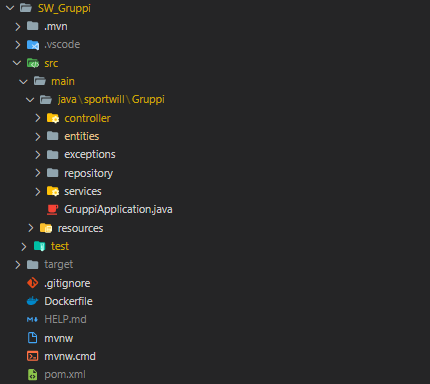
\includegraphics[width=0.65\columnwidth]{organizzazione_codice_spring.png} 
    \caption{Organizzazione del codice}
\end{figure}
Per inizializzare un nuovo \gls{microservizio} viene utilizzata l'estensione \textbf{Spring Initializr} per Visual Studio Code, che permette la generazione di un progetto per Spring Boot.\\
La cartella che contiene il codice del \gls{microservizio} è \texttt{src\textbackslash main\textbackslash java\textbackslash sportwill\textbackslash Gruppi}, che contiene le seguenti cartelle: 
\begin{itemize}
    \item \texttt{controller}: contiene la classe che mappa le richieste HTTP ai metodi specifici;
    \item \texttt{entities}: contiene le classi entità, ovvero classi che rappresentano delle tabelle in un \textit{database} relazionale e ogni istanza di entità corrisponde a una riga in quella tabella;
    \item \texttt{exceptions}: insieme di classi che estendono la classe Exception;
    \item \texttt{services}: classi che compongono il \textit{service layer}.


\end{itemize}
% TODO aggiungere alla bibliografia: https://microservices.io/patterns/apigateway.html
\subsubsection{Progettazione delle API}
Il \textit{back-end} del progetto è strutturato a \glspl{microservizio}, ognuno contenente una business logic atta a soddisfare un certo tipo di richieste.\\
Il \textit{front-end} comunica con il \textit{back-end} attraverso gli \gls{endpoint} che ogni \gls{microservizio} espone. \\
Tuttavia, effettuare connessioni dirette fra \textit{front-end} e ogni \gls{microservizio} presenta alcuni problemi, come: 
\begin{itemize}
    \item numerose connessioni a seconda della quantità dei \glspl{microservizio};
    \item i \glspl{microservizio} devono esporre pubblicamente il proprio \gls{IP}, causando problemi sia di sicurezza, dovuta all'esposizione degli indirizzi IP al mondo esterno, sia in fase di latenza, ovvero il tempo che intercorre tra l'invio di una richiesta ed una risposta tenderà ad essere
    sempre più alto.
\end{itemize}

\noindent Per far fronte a queste problematiche si è deciso di utilizzare un \gls{API Gateway}.\\
In questo modo, solamente un \gls{IP} sarà visibile pubblicamente, mentre quelli dei \glspl{microservizio} possono diventare privati.\\
Per quanto riguarda la latenza il \textit{front-end} comunicherà attraverso l'\gls{API Gateway}, stabilendo solo le connessioni per la richiesta e la risposta, lasciando all'\gls{API Gateway} il compito di smistare le richieste al giusto \gls{microservizio}, permettendo una connessione più rapida rispetto  all'utilizzo di connessioni diverse per ogni \gls{microservizio}, essendo tutti all'interno dello stesso \textit{network}.

\subsection{Front-end}
\subsubsection{Architettura Angular}
% TODO aggiungere alla bibliografia: https://angular.io/guide/architecture
Il componente principale di Angular è il \textbf{modulo}. Un modulo è un contenitore di funzionalità che sono esposte ad altri moduli. Questa suddivisione in moduli rende la struttura dell'applicazione ordinata e il codice mantenibile.\\
Un elemento fondamentale di Angular è il \textbf{component}, ovvero delle classi che gestiscono le \textit{view} dell'applicazione e la loro logica.\\
I dati da visualizzare nella \textit{view} vengono forniti dalle classi dette \textbf{servizi}. Queste classi svolgono diverse funzioni, come per esempio  l'esecuzione delle richieste HTTP.\\  
Ad ogni component è associato un \textit{template}, ovvero del codice HTML in cui si definisce come viene visualizzato il component.\\
È possibile personalizzare il codice HTML utilizzando le \textbf{direttive}, ovvero delle classi che aggiungono un comportamento aggiuntivo agli elementi nelle applicazioni Angular. Le direttive integrate di Angular permettono di gestire moduli, elenchi, stili e ciò che gli utenti vedono.\\
È possibile creare un component che rappresenta la pagina completa, in cui inserire diversi component per ogni elemento contenuto in quella pagina.
Ogni component contenuto si occuperà così di gestire la grafica di quella determinata funzionalità e di comunicare con i servizi di cui necessita; sarà poi il component \enquote*{padre} a gestire la disposizione dei component utilizzati. 
\subsubsection{Organizzazione del codice}

\subsubsection{Progettazione delle maschere}
Descrizione Figma e delle scelte realizzative del mockup realizzato.


\subsubsection{Namespace 1} %**************************
Descrizione namespace 1.

\begin{namespacedesc}
    \classdesc{Classe 1}{Descrizione classe 1}
    \classdesc{Classe 2}{Descrizione classe 2}
\end{namespacedesc}


%**************************************************************
\section{Design Pattern utilizzati}
\subsection{Microservizi}
\subsection{Api Gateway}
\subsection{Service Discovery}
\subsection{Service Registry}
\subsection{Dependency Injection}
\subsection{Singleton}
\subsection{Feature Service}
\subsection{Decorator}
\subsection{Lazy Loading}
\subsection{Observer}

%**************************************************************
\section{Codifica}
\subsection{Back-end}

\subsubsection{Gruppi service}
\subsubsection{Modifica dei servizi esistenti}
\subsubsection{Api Gateway ed Eureka Server}
\subsubsection{Docker}

\subsection{Front-end}
\subsubsection{Maschere}
\subsubsection{Componenti}